\documentclass[tikz,border=10pt]{standalone}
\usepackage{tikz}
\usetikzlibrary{arrows.meta,positioning,fit,calc,backgrounds,shapes.geometric}

\begin{document}
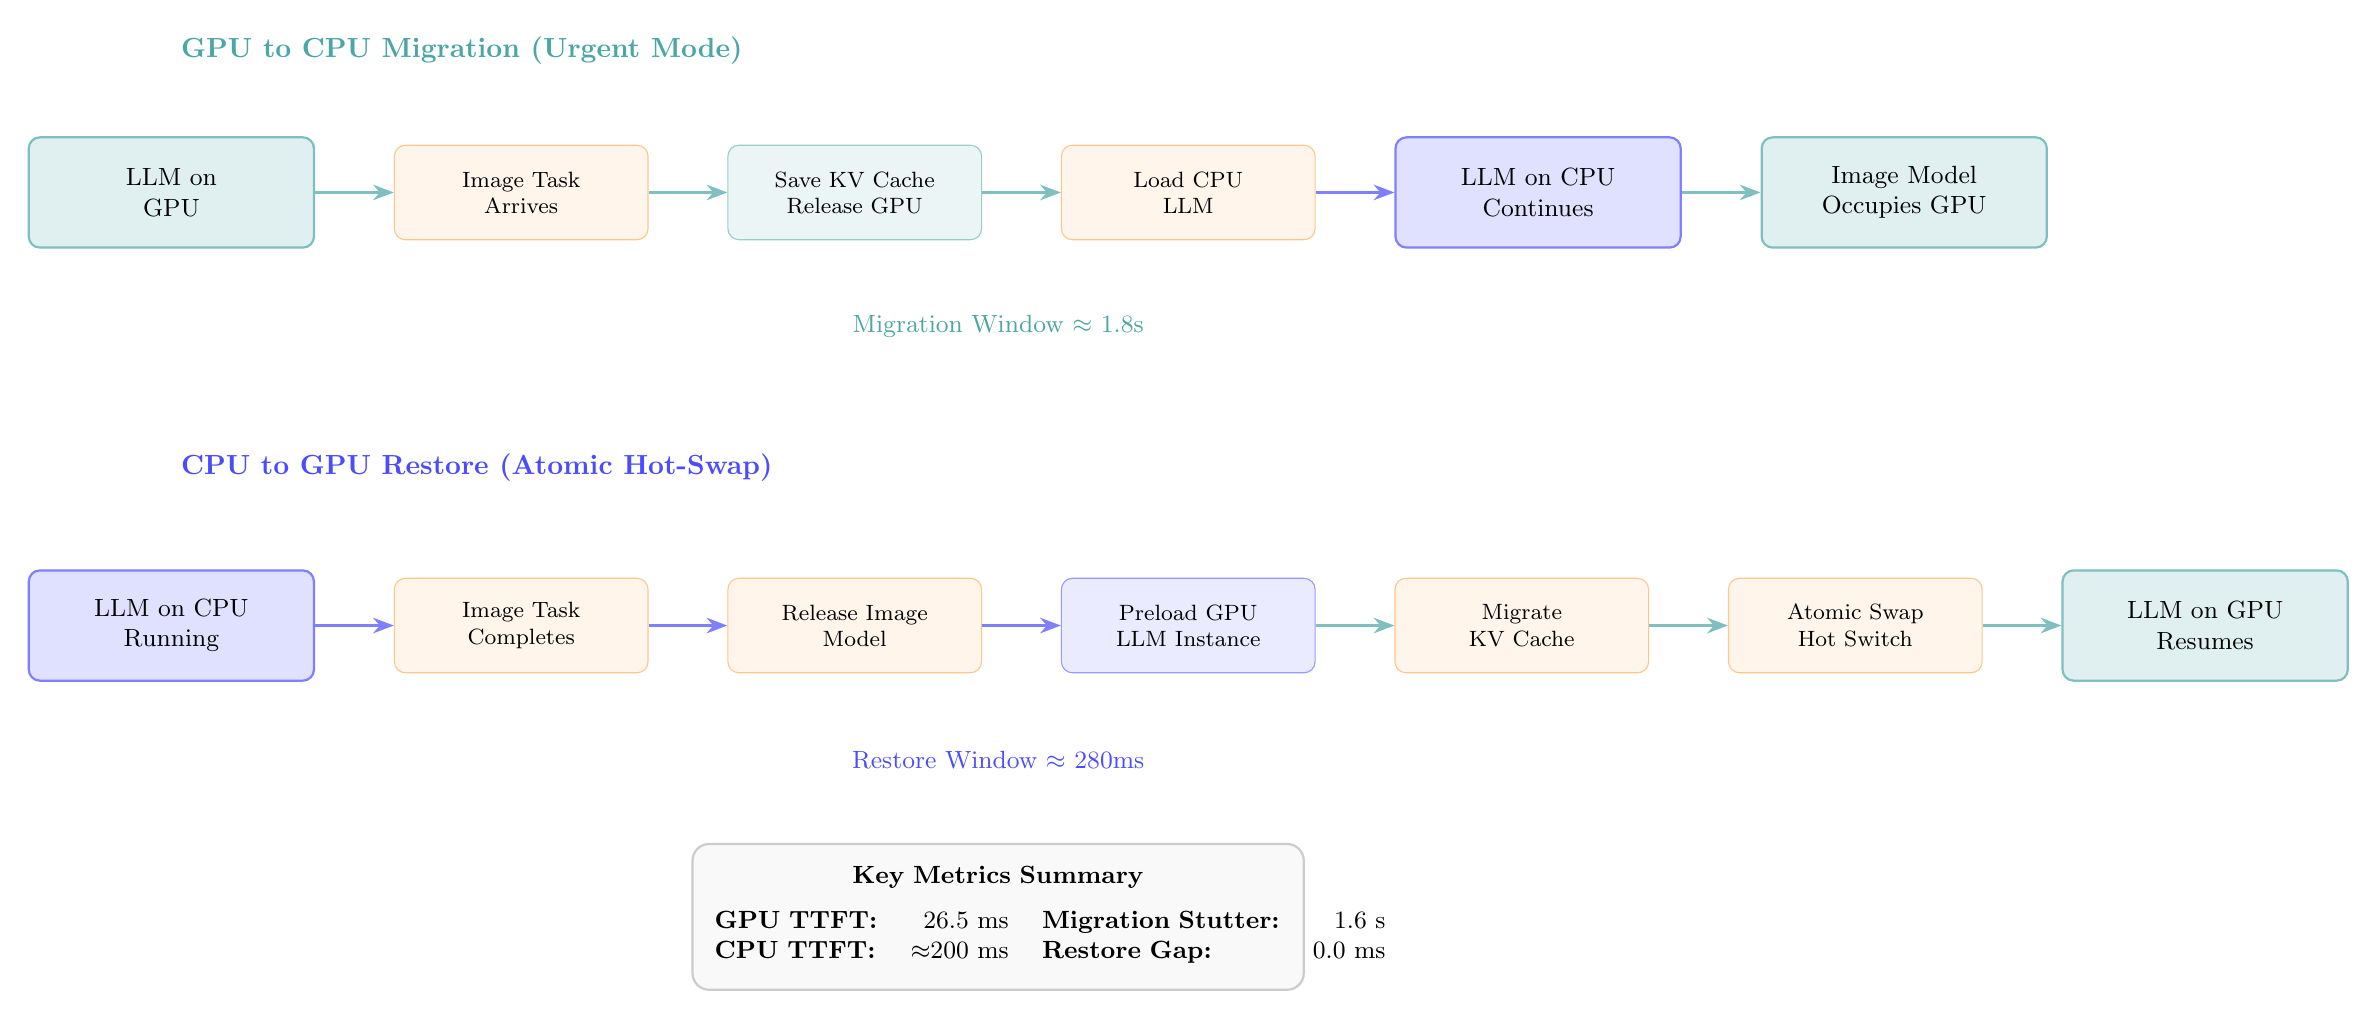
\begin{tikzpicture}[
    font=\small,
    >=Stealth,
    node distance=10mm,
    box/.style={draw, rounded corners=4pt, minimum height=14mm, align=center, inner sep=6pt, text width=32mm, font=\small},
    gpbox/.style={box, fill=teal!12, draw=teal!50, line width=0.8pt},
    cpbox/.style={box, fill=blue!12, draw=blue!50, line width=0.8pt},
    actbox/.style={box, fill=orange!8, draw=orange!45, minimum height=12mm, text width=28mm, font=\footnotesize},
    label/.style={font=\normalsize\bfseries},
    arrow/.style={->, >=Stealth, line width=1pt},
]

% ==================== GPU to CPU Migration Flow ====================
\node[label, text=teal!70, anchor=west] at (0, 5) {\textbf{GPU to CPU Migration (Urgent Mode)}};

% Process boxes
\node[gpbox] (t1) at (0, 3.2) {LLM on\\GPU};
\node[actbox, right=of t1] (t2) {Image Task\\Arrives};
\node[actbox, fill=teal!8, draw=teal!40, right=of t2] (t3) {Save KV Cache\\Release GPU};
\node[actbox, right=of t3] (t4) {Load CPU\\LLM};
\node[cpbox, right=of t4] (t5) {LLM on CPU\\Continues};
\node[gpbox, right=of t5] (t6) {Image Model\\Occupies GPU};

% Arrows
\draw[arrow, draw=teal!50] (t1) -- (t2);
\draw[arrow, draw=teal!50] (t2) -- (t3);
\draw[arrow, draw=teal!50] (t3) -- (t4);
\draw[arrow, draw=blue!50] (t4) -- (t5);
\draw[arrow, draw=teal!50] (t5) -- (t6);

% Migration window annotation (centered, no arrow)
\node[font=\small, text=teal!70] at (10.5, 1.5) {Migration Window $\approx$ 1.8s};

% ==================== CPU to GPU Restore Flow ====================
\node[label, text=blue!70, anchor=west] at (0, -0.3) {\textbf{CPU to GPU Restore (Atomic Hot-Swap)}};

% Process boxes
\node[cpbox] (r1) at (0, -2.3) {LLM on CPU\\Running};
\node[actbox, right=of r1] (r2) {Image Task\\Completes};
\node[actbox, right=of r2] (r3) {Release Image\\Model};
\node[actbox, fill=blue!8, draw=blue!40, right=of r3] (r4) {Preload GPU\\LLM Instance};
\node[actbox, right=of r4] (r5) {Migrate\\KV Cache};
\node[actbox, right=of r5] (r6) {Atomic Swap\\Hot Switch};
\node[gpbox, right=of r6] (r7) {LLM on GPU\\Resumes};

% Arrows
\draw[arrow, draw=blue!50] (r1) -- (r2);
\draw[arrow, draw=blue!50] (r2) -- (r3);
\draw[arrow, draw=blue!50] (r3) -- (r4);
\draw[arrow, draw=teal!50] (r4) -- (r5);
\draw[arrow, draw=teal!50] (r5) -- (r6);
\draw[arrow, draw=teal!50] (r6) -- (r7);

% Restore window annotation (centered, no arrow)
\node[font=\small, text=blue!70] at (10.5, -4.0) {Restore Window $\approx$ 280ms};

% ==================== Key Metrics (Centered) ====================
\node[draw=gray!40, rounded corners=6pt, fill=gray!5, text width=72mm, align=center, font=\small,
      inner sep=8pt, line width=0.8pt] at (10.5, -6.0) {
    \textbf{Key Metrics Summary}\\[2mm]
    \begin{tabular}{@{}l r l r@{}}
    \textbf{GPU TTFT:} & 26.5 ms & \textbf{Migration Stutter:} & 1.6 s \\
    \textbf{CPU TTFT:} & $\approx$200 ms & \textbf{Restore Gap:} & 0.0 ms \\
    \end{tabular}
};

\end{tikzpicture}
\end{document}
